\documentclass[12pt]{article}
\usepackage{amssymb,mathrsfs, amsmath,amsfonts}
\usepackage{mathtools}
\usepackage{graphicx}
\usepackage{enumitem}
\usepackage{braket}
\graphicspath{ {./ps4-assets/}{./exercises/handwritten/ps4-assets/} }


\title{Problem Set 4}
\author{CSE 468}
\date{May 2021}

\begin{document}

\maketitle



\begin{enumerate}[font=\bfseries]
    \item Just some ideas currently. - Will
    \item Give the unitary matrix that describes the below circuit. Note the second gate is the controlled Z gate. Is the state at the end of this circuit entangled? Why or why not?
    \[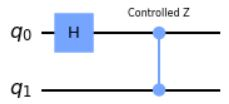
\includegraphics[scale=0.8]{cz-gate}\]
    \item Can the controlled Z gate be factored? Prove or disprove.
    \item Consider the controlled U gate.
    \[\begin{pmatrix}
    1 & 0 & 0 & 0 \\
    0 & e^{i\gamma}\cos{\frac{\theta}{2}} & 0 &  -e^{i(\gamma+\lambda)}\sin{\frac{\theta}{2}}\\
    0 & 0 & 1 & 0 \\
    0 & e^{i(\gamma+\phi)}\sin{\frac{\theta}{2}} & 0 &  e^{i(\gamma+\phi+\lambda)}\cos{\frac{\theta}{2}}\\
    \end{pmatrix}
    \]
    For what values of $\gamma,\phi,\lambda,$ and $\theta$ can we use the controlled U gate to cause entanglement?
    \item Consider standard quantum teleportation. Imagine Alice has the incredible power to transmit exactly one bit to Bob instantaneously (faster than the speed of light whoa). How "well" can Bob do? (What's the probability that Bob obtains the correct state?) (What does Bob know for sure?) (Does it matter which bit Alice chooses to communicate?) (In what situations would Bob prefer to know the first or the second bit of Alice's measurement?)
    \item Prove that using just a single EPR pair, Alice and Bob cannot do better than 50\% without communication and disregarding phase.
    \item Consider the entangled state 
    \[\ket{\psi} = \frac{1}{\sqrt{2}}(\ket{00}+\ket{11})\]
    Show that applying a general U gate to the first qubit still results in an entangled state.
    \item What is the relationship between the factorability of a 2 qubit gate and that same gate's ability to cause entanglement? (I'm not sure)
    \item Recreate the table on slide 9 in slide deck 10 (ie what action Bob should take for each measurement Alice could observe) if Alice and Bob used the below EPR pair to accomplish quantum teleporation.
    \[\ket{\psi} = \frac{1}{\sqrt{2}}(\ket{01}-\ket{10})\]
    \item Partial measurement question? Just easy math question of renormalizing
    
\end{enumerate}



\end{document}